\documentclass{article}\usepackage[]{graphicx}\usepackage[]{color}
%% maxwidth is the original width if it is less than linewidth
%% otherwise use linewidth (to make sure the graphics do not exceed the margin)
\makeatletter
\def\maxwidth{ %
  \ifdim\Gin@nat@width>\linewidth
    \linewidth
  \else
    \Gin@nat@width
  \fi
}
\makeatother

\definecolor{fgcolor}{rgb}{0.345, 0.345, 0.345}
\newcommand{\hlnum}[1]{\textcolor[rgb]{0.686,0.059,0.569}{#1}}%
\newcommand{\hlstr}[1]{\textcolor[rgb]{0.192,0.494,0.8}{#1}}%
\newcommand{\hlcom}[1]{\textcolor[rgb]{0.678,0.584,0.686}{\textit{#1}}}%
\newcommand{\hlopt}[1]{\textcolor[rgb]{0,0,0}{#1}}%
\newcommand{\hlstd}[1]{\textcolor[rgb]{0.345,0.345,0.345}{#1}}%
\newcommand{\hlkwa}[1]{\textcolor[rgb]{0.161,0.373,0.58}{\textbf{#1}}}%
\newcommand{\hlkwb}[1]{\textcolor[rgb]{0.69,0.353,0.396}{#1}}%
\newcommand{\hlkwc}[1]{\textcolor[rgb]{0.333,0.667,0.333}{#1}}%
\newcommand{\hlkwd}[1]{\textcolor[rgb]{0.737,0.353,0.396}{\textbf{#1}}}%

\usepackage{framed}
\makeatletter
\newenvironment{kframe}{%
 \def\at@end@of@kframe{}%
 \ifinner\ifhmode%
  \def\at@end@of@kframe{\end{minipage}}%
  \begin{minipage}{\columnwidth}%
 \fi\fi%
 \def\FrameCommand##1{\hskip\@totalleftmargin \hskip-\fboxsep
 \colorbox{shadecolor}{##1}\hskip-\fboxsep
     % There is no \\@totalrightmargin, so:
     \hskip-\linewidth \hskip-\@totalleftmargin \hskip\columnwidth}%
 \MakeFramed {\advance\hsize-\width
   \@totalleftmargin\z@ \linewidth\hsize
   \@setminipage}}%
 {\par\unskip\endMakeFramed%
 \at@end@of@kframe}
\makeatother

\definecolor{shadecolor}{rgb}{.97, .97, .97}
\definecolor{messagecolor}{rgb}{0, 0, 0}
\definecolor{warningcolor}{rgb}{1, 0, 1}
\definecolor{errorcolor}{rgb}{1, 0, 0}
\newenvironment{knitrout}{}{} % an empty environment to be redefined in TeX

\usepackage{alltt}

\usepackage{amsmath, amssymb}
\usepackage{graphicx}
\usepackage{hyperref}
\IfFileExists{upquote.sty}{\usepackage{upquote}}{}
\begin{document}

\title{Pol Sci 630:  Problem Set 8 Solutions: Dummy Variables and Interactions (Part 2)}

\author{Prepared by: Anh Le (\href{mailto:anh.le@duke.edu}{anh.le@duke.edu})}

\date{Due Date: Friday, Oct 23, 2015, 12 AM (Beginning of Lab)}

\maketitle

\section{Interaction (8 points)}

\textbf{\color{red} Insert your comments on the assignment that you are grading above the solution in bold and red text. For example write: "GRADER COMMENT: everything is correct! - 8/8 Points" Also briefly point out which, if any, problems were not solved correctly and what the mistake was. See below for more examples.}

\subsection*{a)}

Download FDI, tariff, and GDP data from WDI for all countries, year 2010 (\verb`indicator = c("BX.KLT.DINV.CD.WD", "TM.TAX.MRCH.SM.AR.ZS", "NY.GDP.MKTP.CD")`). Clean the data as usual. Run the following regression, showing a stargazer result table.

\begin{align}
\log(FDI) &= \beta_0 + \beta_1 tariff + \beta_2 \log(gdp) + \beta_3 tariff \times \log(gdp)
\end{align}

\textbf{Solution}

\begin{knitrout}
\definecolor{shadecolor}{rgb}{0.969, 0.969, 0.969}\color{fgcolor}\begin{kframe}
\begin{alltt}
\hlkwd{library}\hlstd{(WDI)}
\hlkwd{library}\hlstd{(dplyr)}

\hlstd{d_wdi_raw} \hlkwb{<-} \hlkwd{WDI}\hlstd{(}\hlkwc{indicator} \hlstd{=} \hlkwd{c}\hlstd{(}\hlstr{"BX.KLT.DINV.CD.WD"}\hlstd{,} \hlstr{"TM.TAX.MRCH.SM.AR.ZS"}\hlstd{,}
                               \hlstr{"NY.GDP.MKTP.CD"}\hlstd{),}
         \hlkwc{start} \hlstd{=} \hlnum{2010}\hlstd{,} \hlkwc{end} \hlstd{=} \hlnum{2010}\hlstd{,} \hlkwc{extra} \hlstd{=} \hlnum{TRUE}\hlstd{)}

\hlcom{# Cleaning data with dplyr (rename variables, remove aggregate, log transform)}
\hlcom{# Hope its nice syntax motivates you to learn this package}
\hlstd{d_wdi} \hlkwb{<-} \hlstd{d_wdi_raw} \hlopt
  \hlkwd{rename}\hlstd{(}\hlkwc{fdi} \hlstd{= BX.KLT.DINV.CD.WD,}
         \hlkwc{tariff} \hlstd{= TM.TAX.MRCH.SM.AR.ZS,}
         \hlkwc{gdp} \hlstd{= NY.GDP.MKTP.CD)} \hlopt
  \hlkwd{filter}\hlstd{(region} \hlopt{!=} \hlstr{"Aggregates"}\hlstd{)} \hlopt
  \hlkwd{mutate}\hlstd{(}\hlkwc{loggdp} \hlstd{=} \hlkwd{log}\hlstd{(gdp),} \hlkwc{logfdi} \hlstd{=} \hlkwd{log}\hlstd{(fdi))}
\end{alltt}


{\ttfamily\noindent\color{warningcolor}{\#\# Warning in mutate\_impl(.data, dots): NaNs produced}}\begin{alltt}
\hlstd{m1} \hlkwb{<-} \hlkwd{lm}\hlstd{(logfdi} \hlopt{~} \hlstd{tariff} \hlopt{+} \hlstd{loggdp} \hlopt{+} \hlstd{tariff}\hlopt{:}\hlstd{loggdp,} \hlkwc{data} \hlstd{= d_wdi)}
\end{alltt}
\end{kframe}
\end{knitrout}

\begin{kframe}
\begin{alltt}
\hlkwd{library}\hlstd{(stargazer)}
\end{alltt}


{\ttfamily\noindent\itshape\color{messagecolor}{\#\# \\\#\# Please cite as: \\\#\# \\\#\#\ \ Hlavac, Marek (2014). stargazer: LaTeX code and ASCII text for well-formatted regression and summary statistics tables.\\\#\#\ \ R package version 5.1. http://CRAN.R-project.org/package=stargazer}}\begin{alltt}
\hlkwd{stargazer}\hlstd{(m1)}
\end{alltt}
\end{kframe}
% Table created by stargazer v.5.1 by Marek Hlavac, Harvard University. E-mail: hlavac at fas.harvard.edu
% Date and time: Fri, Oct 16, 2015 - 12:07:40 AM
\begin{table}[!htbp] \centering 
  \caption{} 
  \label{} 
\begin{tabular}{@{\extracolsep{5pt}}lc} 
\\[-1.8ex]\hline 
\hline \\[-1.8ex] 
 & \multicolumn{1}{c}{\textit{Dependent variable:}} \\ 
\cline{2-2} 
\\[-1.8ex] & logfdi \\ 
\hline \\[-1.8ex] 
 tariff & 0.141 \\ 
  & (0.313) \\ 
  & \\ 
 loggdp & 0.930$^{***}$ \\ 
  & (0.101) \\ 
  & \\ 
 tariff:loggdp & $-$0.008 \\ 
  & (0.013) \\ 
  & \\ 
 Constant & $-$1.537 \\ 
  & (2.556) \\ 
  & \\ 
\hline \\[-1.8ex] 
Observations & 108 \\ 
R$^{2}$ & 0.761 \\ 
Adjusted R$^{2}$ & 0.754 \\ 
Residual Std. Error & 1.287 (df = 104) \\ 
F Statistic & 110.431$^{***}$ (df = 3; 104) \\ 
\hline 
\hline \\[-1.8ex] 
\textit{Note:}  & \multicolumn{1}{r}{$^{*}$p$<$0.1; $^{**}$p$<$0.05; $^{***}$p$<$0.01} \\ 
\end{tabular} 
\end{table} 


\subsection*{b)}

Mathematically, what is the marginal effect of tariff on logfdi (i.e. taking partial derivative)? Plugging in the number, what's the marginal effect of tariff on logfdi, holding loggdp at its median value? Note: Use \verb`\Sexpr()` to extract coefficients from the model, do not hand write your calculation.

\textbf{Solution}

\begin{align}
\frac{\partial}{\partial tariff} logfdi &= \beta_1 + \beta_3 loggdp
\end{align}

The median value of loggdp is 23.8854648

The marginal effect of tariff, holding loggdp at its median value, is \ensuremath{-0.0437074}

\subsection*{c)}

Using \verb`ggplot2`, plot the marginal effect of tariff on logfdi (y-axis) against different values of loggdp (x-axis). (Hint: Create a data frame, in which one variable is the values of loggdp, the other variable is the corresponding marginal effect given that value of loggdp. This data frame is the data that makes up your plot. The plot is just a line.)

\textbf{Solution}

\begin{knitrout}
\definecolor{shadecolor}{rgb}{0.969, 0.969, 0.969}\color{fgcolor}\begin{kframe}
\begin{alltt}
\hlkwd{library}\hlstd{(ggplot2)}
\hlcom{# pd is my shorthand for plot data}
\hlstd{loggdp} \hlkwb{<-} \hlkwd{sort}\hlstd{(d_wdi}\hlopt{$}\hlstd{loggdp)}
\hlstd{marginaleffect} \hlkwb{<-} \hlstd{m1}\hlopt{$}\hlstd{coefficients[}\hlstr{'tariff'}\hlstd{]} \hlopt{+} \hlstd{loggdp} \hlopt{*} \hlstd{m1}\hlopt{$}\hlstd{coefficients[}\hlstr{'tariff:loggdp'}\hlstd{]}
\hlstd{pd} \hlkwb{<-} \hlkwd{data.frame}\hlstd{(}\hlkwc{loggdp} \hlstd{= loggdp,}
                 \hlkwc{marginaleffect} \hlstd{= marginaleffect)}

\hlkwd{ggplot}\hlstd{(}\hlkwc{data} \hlstd{= pd)} \hlopt{+}
  \hlkwd{geom_line}\hlstd{(}\hlkwd{aes}\hlstd{(}\hlkwc{x} \hlstd{= loggdp,} \hlkwc{y} \hlstd{= marginaleffect))} \hlopt{+}
  \hlkwd{labs}\hlstd{(}\hlkwc{y} \hlstd{=} \hlstr{"Marginal effect of tariff on logfdi"}\hlstd{,} \hlkwc{x} \hlstd{=} \hlstr{"log GDP"}\hlstd{)}
\end{alltt}
\end{kframe}
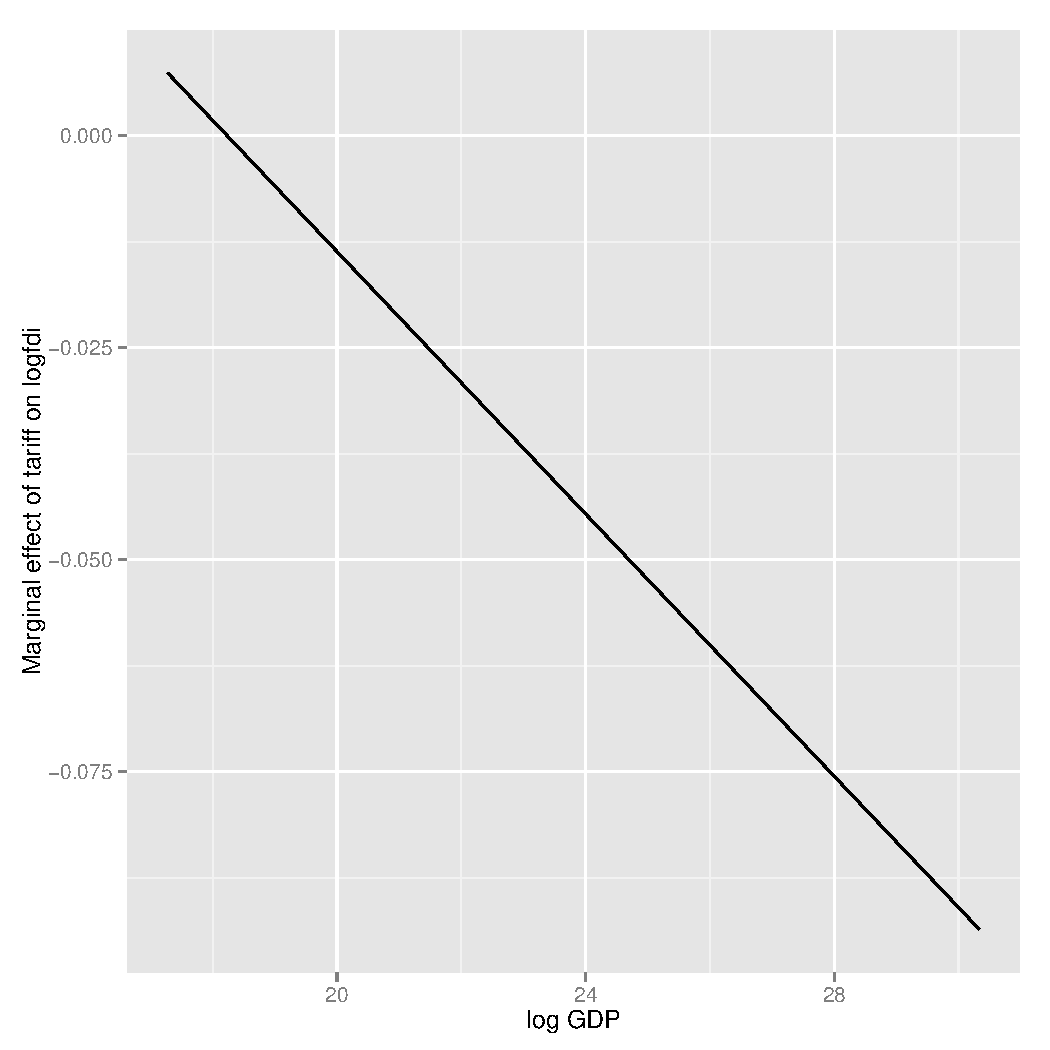
\includegraphics[width=\maxwidth]{figure/unnamed-chunk-3-1} 

\end{knitrout}

\subsection*{d)}

With log fdi on the y-axis, tariff on the x-axis, plot the effect of tariff on log fdi when log gdp is at the 25\%, 50\%, and 75\% percentile.

(Hint: The plot should have 3 lines, each according to a value of log gdp. This is the plot you saw in last lab)

\textbf{Solution}

\begin{knitrout}
\definecolor{shadecolor}{rgb}{0.969, 0.969, 0.969}\color{fgcolor}\begin{kframe}
\begin{alltt}
\hlkwd{library}\hlstd{(dplyr)}
\hlkwd{library}\hlstd{(ggplot2)}

\hlstd{loggdp_quantiles} \hlkwb{<-} \hlkwd{quantile}\hlstd{(d_wdi}\hlopt{$}\hlstd{loggdp,} \hlkwc{probs} \hlstd{=} \hlkwd{c}\hlstd{(}\hlnum{0.25}\hlstd{,} \hlnum{0.5}\hlstd{,} \hlnum{0.75}\hlstd{),} \hlkwc{na.rm}\hlstd{=}\hlnum{TRUE}\hlstd{)}


\hlstd{newdata} \hlkwb{<-} \hlkwd{data.frame}\hlstd{(}\hlkwc{tariff} \hlstd{=} \hlkwd{rep}\hlstd{(d_wdi}\hlopt{$}\hlstd{tariff,} \hlkwc{times} \hlstd{=} \hlnum{3}\hlstd{),}
                 \hlkwc{loggdp} \hlstd{=} \hlkwd{rep}\hlstd{(loggdp_quantiles,} \hlkwc{each} \hlstd{=} \hlkwd{nrow}\hlstd{(d_wdi)))}
\hlstd{pred} \hlkwb{<-} \hlkwd{predict}\hlstd{(m1,} \hlkwc{newdata} \hlstd{= newdata,} \hlkwc{se.fit} \hlstd{=} \hlnum{TRUE}\hlstd{)}

\hlstd{pd} \hlkwb{<-} \hlstd{newdata} \hlopt
  \hlkwd{mutate}\hlstd{(}\hlkwc{logfdi} \hlstd{= pred}\hlopt{$}\hlstd{fit,}
         \hlkwc{ymin} \hlstd{= logfdi} \hlopt{-} \hlnum{1.96} \hlopt{*} \hlstd{pred}\hlopt{$}\hlstd{se.fit,}
         \hlkwc{ymax} \hlstd{= logfdi} \hlopt{+} \hlnum{1.96} \hlopt{*} \hlstd{pred}\hlopt{$}\hlstd{se.fit)}
\hlkwd{ggplot}\hlstd{(}\hlkwc{data} \hlstd{= pd)} \hlopt{+}
  \hlkwd{geom_line}\hlstd{(}\hlkwd{aes}\hlstd{(}\hlkwc{x} \hlstd{= tariff,} \hlkwc{y} \hlstd{= logfdi,} \hlkwc{color} \hlstd{=} \hlkwd{factor}\hlstd{(loggdp)))} \hlopt{+}
  \hlkwd{geom_ribbon}\hlstd{(}\hlkwd{aes}\hlstd{(}\hlkwc{x} \hlstd{= tariff,} \hlkwc{ymin} \hlstd{= ymin,} \hlkwc{ymax} \hlstd{= ymax,}
                  \hlkwc{color} \hlstd{=} \hlkwd{factor}\hlstd{(loggdp)),} \hlkwc{alpha} \hlstd{=} \hlnum{0.3}\hlstd{)} \hlopt{+}
  \hlkwd{labs}\hlstd{(}\hlkwc{title} \hlstd{=} \hlstr{"The effect of tariff on log fdi for different values of log FDI"}\hlstd{)} \hlopt{+}
  \hlkwd{scale_color_discrete}\hlstd{(}\hlkwc{name} \hlstd{=} \hlstr{'log GDP'}\hlstd{,}
                       \hlkwc{labels} \hlstd{=} \hlkwd{c}\hlstd{(}\hlstr{'25 percentile'}\hlstd{,} \hlstr{'50 percentile'}\hlstd{,} \hlstr{'75 percentile'}\hlstd{))}
\end{alltt}


{\ttfamily\noindent\color{warningcolor}{\#\# Warning: Removed 282 rows containing missing values (geom\_path).}}\end{kframe}
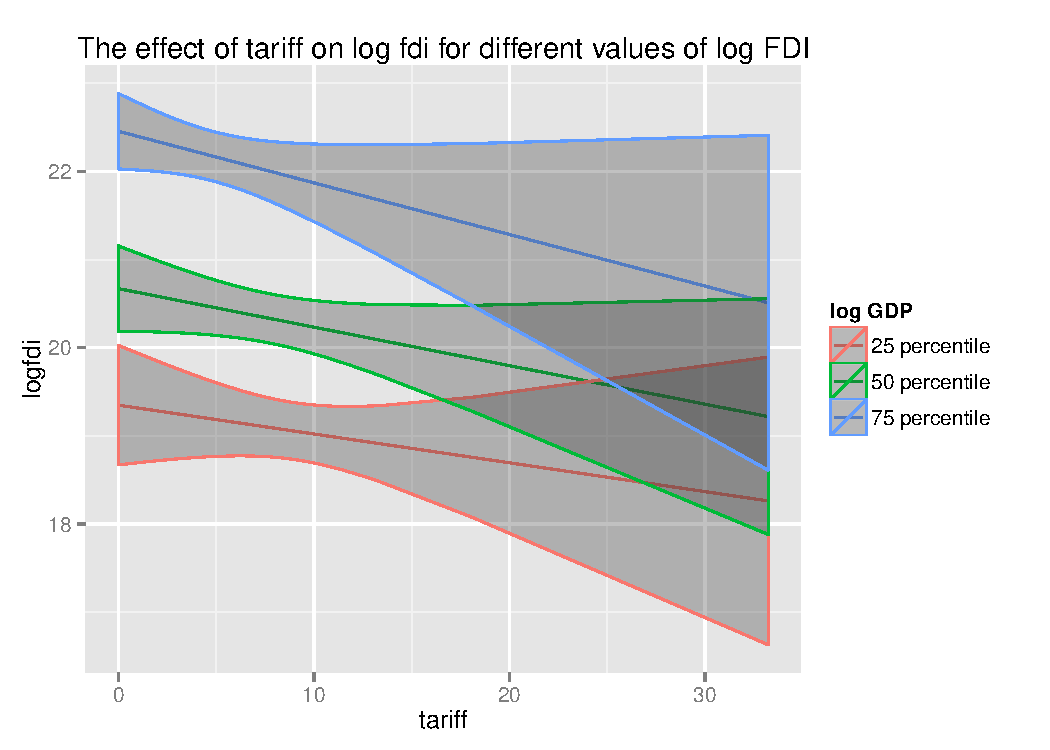
\includegraphics[width=\maxwidth]{figure/unnamed-chunk-4-1} 

\end{knitrout}

\section{Plotting the world with ggplot2 (4 points)}

Plot the world map with \verb`ggplot2`.

If you got stuck, read this \href{http://stackoverflow.com/questions/9805895/mapping-the-world-on-ggplot2}{SO answer} and explain each line of code.

If you encounter the \verb`Error: isTRUE(gpclibPermitStatus()) is not TRUE` error, follow the top answer \href{http://stackoverflow.com/questions/30790036/error-istruegpclibpermitstatus-is-not-true}{here}

\textbf{Solution}

\begin{knitrout}
\definecolor{shadecolor}{rgb}{0.969, 0.969, 0.969}\color{fgcolor}\begin{kframe}
\begin{alltt}
\hlkwd{library}\hlstd{(ggplot2)}
\hlkwd{library}\hlstd{(cshapes)}
\hlkwd{gpclibPermit}\hlstd{()}
\end{alltt}


{\ttfamily\noindent\color{warningcolor}{\#\# Warning in gpclibPermit(): support for gpclib will be withdrawn from maptools at the next major release}}\begin{verbatim}
## [1] TRUE
\end{verbatim}
\begin{alltt}
\hlcom{# Load the shape file of the world data}
\hlstd{world} \hlkwb{<-} \hlkwd{cshp}\hlstd{(}\hlkwc{date}\hlstd{=}\hlkwd{as.Date}\hlstd{(}\hlstr{"2008-1-1"}\hlstd{))}

\hlcom{# Transform the shape file into a data frame}
\hlstd{world.points} \hlkwb{<-} \hlkwd{fortify}\hlstd{(world,} \hlkwc{region}\hlstd{=}\hlstr{'COWCODE'}\hlstd{)}

\hlcom{# Plot the data in the data frame, with mapping}
\hlcom{# longitude -> x-axis, latitude -> y-axis}
\hlcom{# and grouping so that the points that define a country stays together in a group}
\hlstd{p} \hlkwb{<-} \hlkwd{ggplot}\hlstd{(world.points,} \hlkwd{aes}\hlstd{(long, lat,} \hlkwc{group}\hlstd{=group))} \hlopt{+} \hlkwd{geom_polygon}\hlstd{()} \hlopt{+}
  \hlkwd{labs}\hlstd{(}\hlkwc{title} \hlstd{=} \hlstr{"World map"}\hlstd{)}
\hlstd{p}
\end{alltt}
\end{kframe}
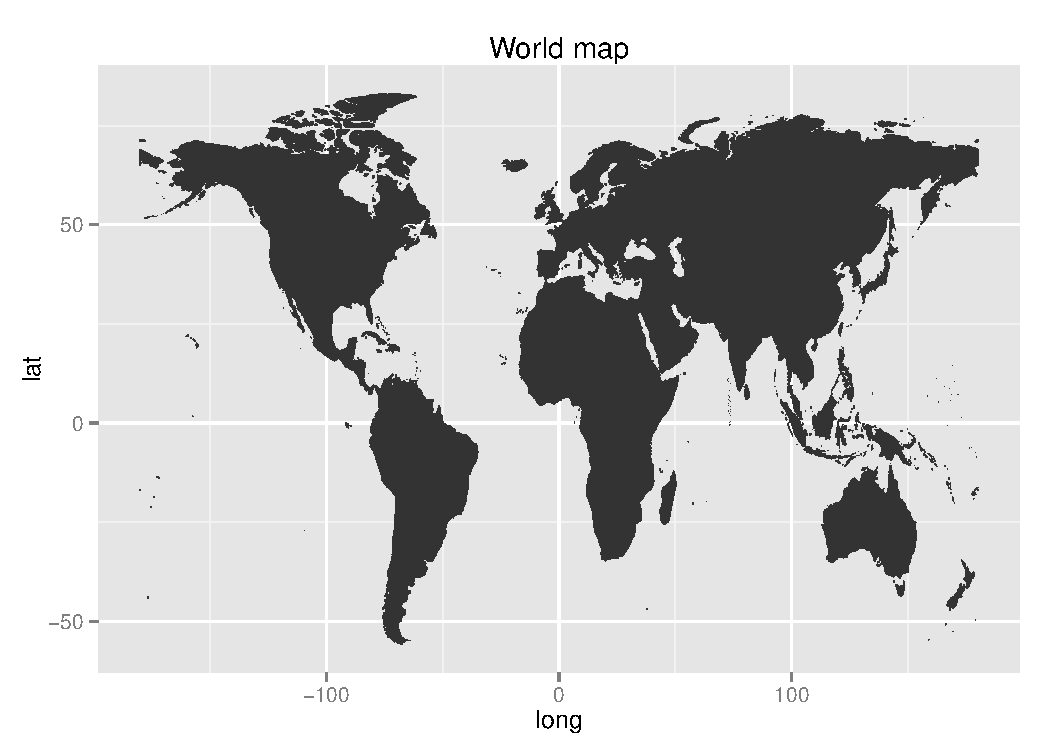
\includegraphics[width=\maxwidth]{figure/unnamed-chunk-5-1} 

\end{knitrout}

\section{ANOVA (4 points)}

Load the diamond dataset in R (\verb`data(diamonds)). With \verb`price` as the dependent variable, run 1) one-way ANOVA on \verb`cut`; 2) two-way ANOVA on \verb`cut` and \verb`clarity` and their interaction.

Interpret the table (i.e. which factor is important in determining the diamond's price?)

\textbf{Solution}

\begin{knitrout}
\definecolor{shadecolor}{rgb}{0.969, 0.969, 0.969}\color{fgcolor}\begin{kframe}
\begin{alltt}
\hlkwd{data}\hlstd{(}\hlstr{"diamonds"}\hlstd{)}
\hlkwd{summary}\hlstd{(}\hlkwd{aov}\hlstd{(price} \hlopt{~} \hlstd{cut,} \hlkwc{data} \hlstd{= diamonds))}
\end{alltt}
\begin{verbatim}
##                Df    Sum Sq   Mean Sq F value Pr(>F)    
## cut             4 1.104e+10 2.760e+09   175.7 <2e-16 ***
## Residuals   53935 8.474e+11 1.571e+07                   
## ---
## Signif. codes:  0 '***' 0.001 '**' 0.01 '*' 0.05 '.' 0.1 ' ' 1
\end{verbatim}
\end{kframe}
\end{knitrout}

\verb`Cut` is a significant factor, judging from the large F-stat and small p-value

\begin{knitrout}
\definecolor{shadecolor}{rgb}{0.969, 0.969, 0.969}\color{fgcolor}\begin{kframe}
\begin{alltt}
\hlkwd{summary}\hlstd{(}\hlkwd{aov}\hlstd{(price} \hlopt{~} \hlstd{cut} \hlopt{+} \hlstd{clarity} \hlopt{+} \hlstd{cut}\hlopt{:}\hlstd{clarity,} \hlkwc{data} \hlstd{= diamonds))}
\end{alltt}
\begin{verbatim}
##                Df    Sum Sq   Mean Sq F value Pr(>F)    
## cut             4 1.104e+10 2.760e+09 180.157 <2e-16 ***
## clarity         7 1.891e+10 2.701e+09 176.305 <2e-16 ***
## cut:clarity    28 2.647e+09 9.452e+07   6.169 <2e-16 ***
## Residuals   53900 8.259e+11 1.532e+07                   
## ---
## Signif. codes:  0 '***' 0.001 '**' 0.01 '*' 0.05 '.' 0.1 ' ' 1
\end{verbatim}
\end{kframe}
\end{knitrout}

\verb`cut`, \verb`clarity`, and their interaction are all important factors in determining the price of diamond.

\end{document}
